\chapter{Множества, логика и доказательства}\markright{Глава 16}
\begin{definition}\term{Множество} (\emph{set}) — совокупность элементов. Запись \(x \in  A\) означает, что \(x\) принадлежит множеству \(A\).\end{definition}
\begin{definition}\term{Пересечение} (\emph{intersection}) \(A\cap B\) — множество элементов, принадлежащих одновременно \(A\) и \(B\).\end{definition}
\begin{definition}\term{Объединение} (\emph{union}) \(A\cup B\) — множество элементов, принадлежащих хотя бы одному из множеств \(A\) и \(B\).\end{definition}
\begin{definition}\term{Утверждение} (\emph{statement; proposition}) — высказывание, для которого можно определить истинность или ложность в заданных условиях.\end{definition}
\begin{definition}\term{Импликация} (\emph{implication}) \(P\Rightarrow Q\) — высказывание «если \(P\), то \(Q\)».\end{definition}
\begin{definition}\term{Достаточное условие} (\emph{sufficient condition}) для \(Q\) — условие \(P\), из которого следует \(Q\), то есть импликация \(P\Rightarrow Q\) истинна.\end{definition}
\begin{definition}\term{Необходимое условие} (\emph{necessary condition}) для \(P\) — условие \(Q\), которое обязательно выполняется при выполнении \(P\), то есть импликация \(P\Rightarrow Q\) истинна.\end{definition}
\section*{Кванторы и отрицание}
\par\addvspace{5pt}\begin{lrbox}{\CatFlowBox}\begin{minipage}[t]{\linewidth}
\setlength{\parskip}{5pt}\setlength{\columnsep}{4.5mm}\setlength{\intextsep}{0pt}
\begin{wrapfigure}[12]{r}{54mm}

\includegraphics[width=54mm,height=58mm,keepaspectratio]{images/unique/art-23.png}
\end{wrapfigure}
\(\forall \) означает «для любого», \(\exists \) — «существует». \(\mathbb{Z}\) обозначает целые числа, \(\mathbb{R}\) — действительные.\par
Отрицание «для всех \(x\) верно \(P (x)\)» — «существует \(x\), для которого \(P (x)\) неверно».\par
Чтобы опровергнуть всеобщее утверждение, достаточно одного контрпримера. Чтобы доказать его, проверки нескольких примеров недостаточно.\par
\par\WFclear\end{minipage}\end{lrbox}%
\ifdim\dimexpr\ht\CatFlowBox+\dp\CatFlowBox\relax<64mm\dp\CatFlowBox=\dimexpr64mm-\ht\CatFlowBox\relax\fi%
\noindent\usebox{\CatFlowBox}\par\addvspace{5pt}
\section*{Свойства и способы доказательства}
Для конечных множеств: \(| A \cup  B | = | A | + | B | - | A \cap  B |\). Здесь \(| A |\) означает число элементов множества, а не модуль числа.\par
\begin{definition}\term{Контрапозиция} (\emph{contrapositive}) импликации \(P\Rightarrow Q\) — импликация \(\neg Q\Rightarrow\neg P\), равносильная исходной:\[ (P\Rightarrow Q)\Longleftrightarrow(\neg Q\Rightarrow\neg P). \] Здесь \(\neg\) означает отрицание.\end{definition}
Обратное утверждение \(Q\Rightarrow P\) в общем случае из \(P\Rightarrow Q\) не следует.\par
Принцип математической индукции: проверь утверждение для \(n = 1\); затем для любого \(k \ge  1\) докажи переход от его истинности при \(n = k\) к истинности при \(n = k + 1\). Тогда оно верно для всех натуральных \(n \ge  1\).\par
{\small\textit{Пример прямого доказательства: сумма чётных чисел \(2 m\) и \(2 n\) равна \(2 (m + n)\), поэтому она чётна.}}\par

\section*{Подмножества и операции над множествами}
\begin{definition}\term{Подмножество} (subset) \(A\) множества \(B\) — множество, каждый элемент которого принадлежит \(B\). Обозначение \(A\subseteq B\) допускает равенство \(A=B\).\end{definition}
\begin{definition}\term{Собственное подмножество} (proper subset) — подмножество \(A\subseteq B\), не равное \(B\). Обозначение: \(A\subsetneq B\).\end{definition}
\begin{definition}\term{Пустое множество} (empty set) \(\varnothing\) — множество, не содержащее ни одного элемента. Оно является подмножеством любого множества; \(\{\varnothing\}\) содержит один элемент и не равно \(\varnothing\).\end{definition}
\begin{definition}\term{Универсальное множество} (universal set) \(U\) — заранее выбранное множество всех объектов, рассматриваемых в данной задаче. Если говорится о дополнениях, все обсуждаемые множества считаются подмножествами \(U\).\end{definition}
\begin{definition}\term{Разность множеств} (set difference) \(A\setminus B\) — множество элементов, которые принадлежат \(A\), но не принадлежат \(B\).\end{definition}
\begin{definition}\term{Дополнение множества} (complement) \(A\subseteq U\) относительно \(U\) — множество \(U\setminus A\). Без указания \(U\) дополнение может быть неоднозначным.\end{definition}
\begin{definition}\term{Симметрическая разность} (symmetric difference) \(A\triangle B\) — множество элементов, принадлежащих ровно одному из множеств \(A,B\): \(A\triangle B=(A\setminus B)\cup(B\setminus A)\).\end{definition}
\begin{definition}\term{Множество всех подмножеств} (power set) множества \(A\) — множество \(\mathcal P(A)=\{B:B\subseteq A\}\). Например, \(\mathcal P(\{a\})=\{\varnothing,\{a\}\}\).\end{definition}
\begin{definition}\term{Упорядоченная пара} (ordered pair) \((a,b)\) — пара с выделенными первой и второй координатами: \((a,b)=(c,d)\) тогда и только тогда, когда \(a=c\) и \(b=d\).\end{definition}
\begin{definition}\term{Декартово произведение} (Cartesian product) \(A\times B\) — множество всех упорядоченных пар \((a,b)\), где \(a\in A\), \(b\in B\). Например, \(\{1,2\}\times\{3\}=\{(1,3),(2,3)\}\).\end{definition}
\begin{definition}\term{Диаграмма Венна} (Venn diagram) — рисунок, на котором универсальное множество изображают областью, обычно прямоугольником, а его подмножества — областями внутри неё. Закрашивание выделяет элементы, удовлетворяющие нужному условию. Диаграмма помогает понять равенство множеств, но общее доказательство удобно проводить через принадлежность произвольного элемента.\end{definition}
\begin{theorem}[Законы де Моргана]
Если \(A,B\subseteq U\), то \(U\setminus(A\cup B)=(U\setminus A)\cap(U\setminus B)\) и \(U\setminus(A\cap B)=(U\setminus A)\cup(U\setminus B)\).
\end{theorem}
\begin{proof}
Возьмём произвольный \(x\in U\). Условие \(x\notin A\cup B\) означает, что \(x\notin A\) и \(x\notin B\), то есть \(x\in(U\setminus A)\cap(U\setminus B)\). Все переходы обратимы, поэтому доказано первое равенство. Условие \(x\notin A\cap B\) означает, что хотя бы одно из условий \(x\in A\), \(x\in B\) не выполнено. Это равносильно \(x\notin A\) или \(x\notin B\), то есть \(x\in(U\setminus A)\cup(U\setminus B)\). Обратимость переходов даёт второе равенство.
\end{proof}
\begin{theorem}[Число подмножеств]
Если конечное множество \(A\) содержит \(n\) элементов, где \(n\ge0\) — целое число, то \(|\mathcal P(A)|=2^n\).
\end{theorem}
\begin{proof}
Проведём индукцию по \(n\). При \(n=0\) множество \(A\) пусто и имеет ровно одно подмножество — \(\varnothing\); это \(1=2^0\). Пусть у множества из \(k\) элементов \(2^k\) подмножеств. При добавлении нового элемента каждое старое подмножество даёт два различных варианта: без нового элемента и с ним. Эти варианты исчерпывают все подмножества нового множества, поэтому их число равно \(2\cdot2^k=2^{k+1}\).
\end{proof}

\Needspace{7\baselineskip}\section*{Задачи}
\begingroup\setlength{\parskip}{3pt}
\noindent\begin{minipage}[t]{\linewidth}\textbf{16.1.} При \(A = \{1,\allowbreak 2,\allowbreak 3\}\) и \(B = \{3,\allowbreak 4\}\) найди \(A \cap  B\) и \(A \cup  B\).\par\end{minipage}\par
\noindent\begin{minipage}[t]{\linewidth}\textbf{16.2.} Запиши символами: для любого действительного \(x\) число \(x^{2}\) неотрицательно.\par\end{minipage}\par
\noindent\begin{minipage}[t]{\linewidth}\textbf{16.3.} Переведи: \(\exists  x \in  \mathbb{Z} : x^{2} = 9\). Верно ли это?\par\end{minipage}\par
\noindent\begin{minipage}[t]{\linewidth}\textbf{16.4.} Верно ли: для любого действительного \(x\) выполнено \(x^{2} > 0\)?\par\end{minipage}\par
\noindent\begin{minipage}[t]{\linewidth}\textbf{16.5.} Запиши отрицание фразы «все числа в наборе положительны».\par\end{minipage}\par
\par\addvspace{5pt}\begin{lrbox}{\CatFlowBox}\begin{minipage}[t]{\linewidth}
\setlength{\parskip}{5pt}\setlength{\columnsep}{4.5mm}\setlength{\intextsep}{0pt}
\begin{wrapfigure}[12]{l}{54mm}
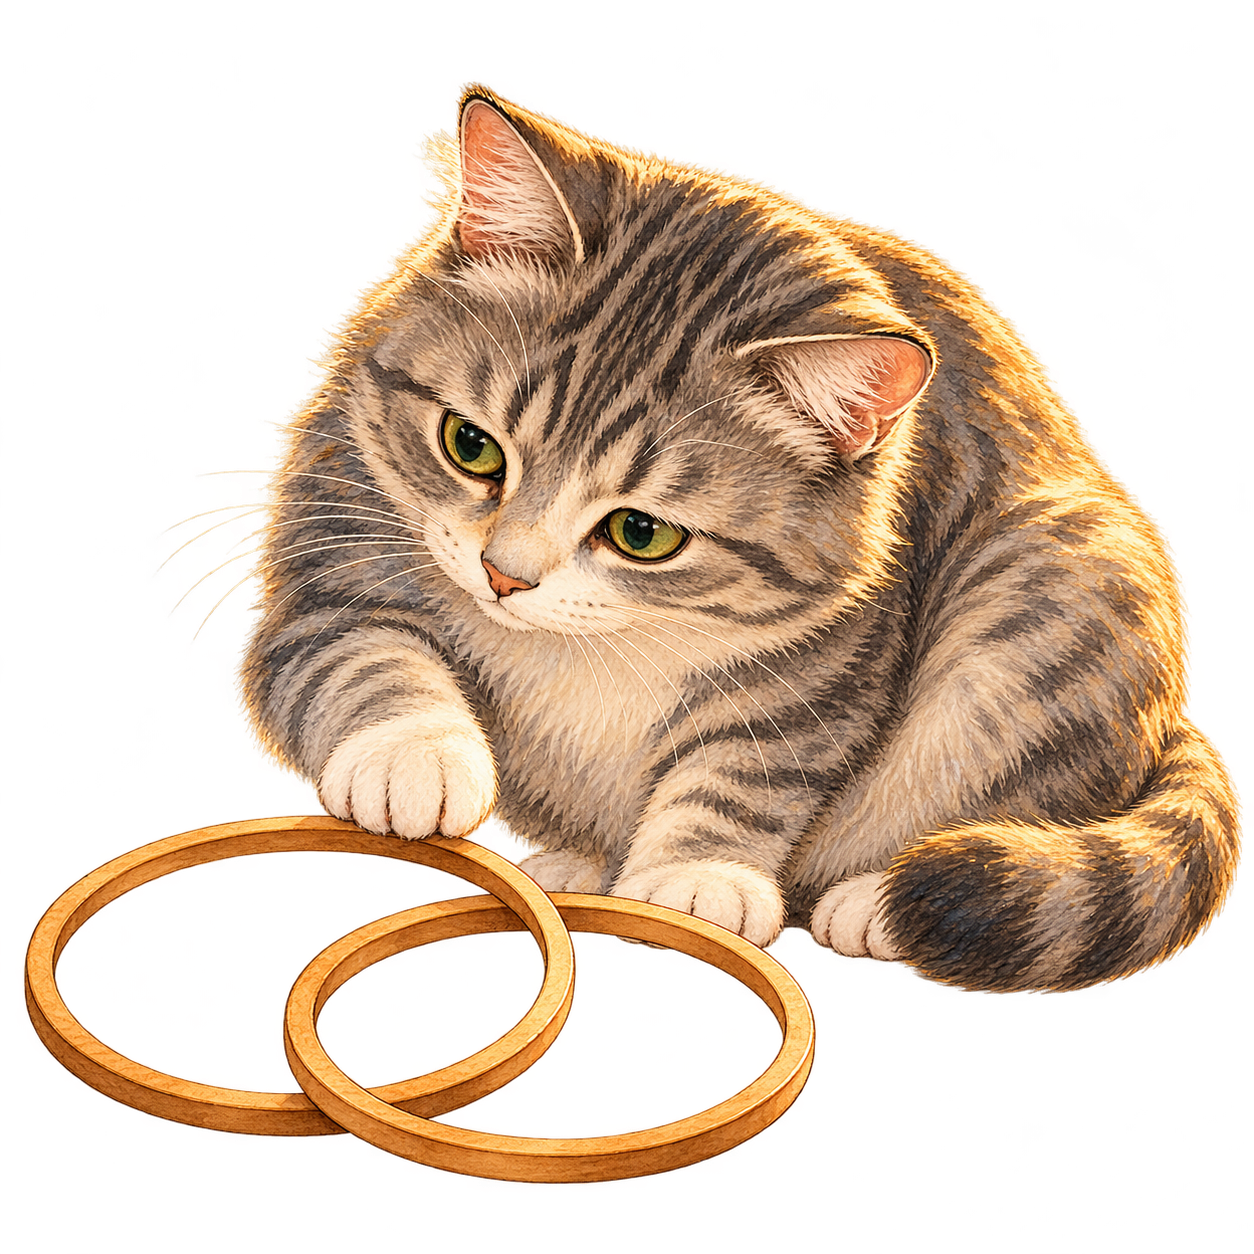
\includegraphics[width=54mm,height=58mm,keepaspectratio]{images/unique/art-32.png}
\end{wrapfigure}
\textbf{16.6.} Верна ли импликация: если число делится на \(4\), то оно чётное? Верно ли обратное?\par

\textbf{16.7.} Для делимости на \(6\) чётность — необходимое или достаточное условие?\par

\textbf{16.8.} Докажи, что сумма двух чётных целых чисел чётна.\par

\textbf{16.9.} Докажи, что квадрат нечётного целого числа нечётный.\par

\textbf{16.10.} Опровергни: если \(a^{2} = b^{2}\), то \(a = b\) для любых действительных \(a,\allowbreak b\).\par

\textbf{16.11.} Докажи по индукции: \(1 + 2 + \ldots  + n = \dfrac{n (n + 1)}{2}\) для натуральных \(n \ge  1\).\par

\textbf{16.12.} Докажи: если целое \(n\) нечётно, то \(n^{2}\) нечётно. Сформулируй равносильное утверждение через противоположное условие.\par
\par\WFclear\end{minipage}\end{lrbox}%
\ifdim\dimexpr\ht\CatFlowBox+\dp\CatFlowBox\relax<64mm\dp\CatFlowBox=\dimexpr64mm-\ht\CatFlowBox\relax\fi%
\noindent\usebox{\CatFlowBox}\par\addvspace{5pt}

\noindent\begin{minipage}[t]{\linewidth}\textbf{16.13.} Из жизни. В кафе все комплексные обеды включают напиток. Покупатель получил напиток. Обязательно ли он заказал комплексный обед?\par\end{minipage}\par
\noindent\begin{minipage}[t]{\linewidth}\textbf{16.14.} Из жизни. В группе \(20\) человек. Чай любят \(12\), кофе любят \(9\), оба напитка любят \(5\). Сколько любят хотя бы один из напитков и сколько не любят ни один?\par\end{minipage}\par
\noindent\begin{minipage}[t]{\linewidth}\textbf{16.15.} Из жизни. Объявление гласит: «Все автобусы на этом маршруте низкопольные». Какое наблюдение опровергнет утверждение? Сформулируй его отрицание.\par\end{minipage}\par
\noindent\begin{minipage}[t]{\linewidth}\textbf{16.16.}\starmark{} Из \(30\) учеников \(18\) изучают английский, \(16\) немецкий, каждый изучает хотя бы один из этих языков. Сколько изучают оба и сколько только английский?\begin{center}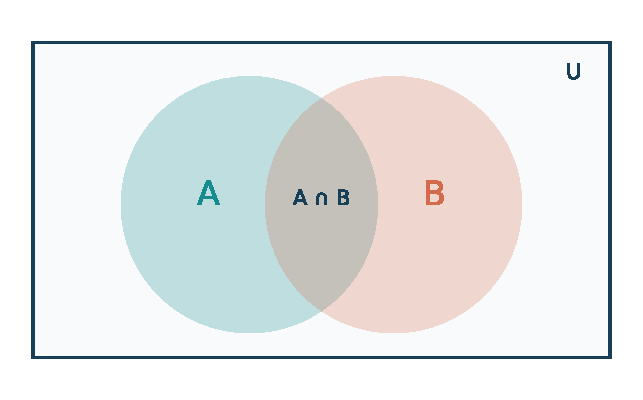
\includegraphics[width=.7\linewidth,height=45mm,keepaspectratio]{images/diagram-venn.pdf}\end{center}\par\end{minipage}\par
\noindent\begin{minipage}[t]{\linewidth}\textbf{16.17.}\starmark{} Докажи: если квадрат целого числа делится на \(3\), то само число делится на \(3\).\par\end{minipage}\par
\noindent\begin{minipage}[t]{\linewidth}\textbf{16.18.}\starmark{} Докажи по индукции: \(1 + 3 + 5 + \ldots  + (2 n - 1) = n^{2}\) для \(n \ge  1\).\par\end{minipage}\par
\noindent\begin{minipage}[t]{\linewidth}\textbf{16.19.}\starmark{} Для \(A,B\subseteq U\) докажи равенство \(A\setminus B=A\cap(U\setminus B)\) через принадлежность произвольного элемента.\par\end{minipage}\par
\noindent\begin{minipage}[t]{\linewidth}\textbf{16.20.}\starmark{} Докажи распределительный закон \(A\cap(B\cup C)=(A\cap B)\cup(A\cap C)\) через принадлежность элемента. Объясни, что нужно закрасить на диаграмме Венна для каждой стороны.\par\end{minipage}\par
\noindent\begin{minipage}[t]{\linewidth}\textbf{16.21.} Пусть \(A=\{1,2\}\), \(B=\{1,2,3\}\), \(C=\{2,4\}\). Определи истинность записей \(A\subseteq B\), \(A\subsetneq B\), \(C\subseteq B\), \(\varnothing\subseteq A\).\par\end{minipage}\par
\noindent\begin{minipage}[t]{\linewidth}\textbf{16.22.} Выпиши все элементы \(\mathcal P(\{a,b\})\), где \(a\ne b\). Сколько подмножеств имеет множество из четырёх элементов?\par\end{minipage}\par
\noindent\begin{minipage}[t]{\linewidth}\textbf{16.23.} Даны \(U=\{1,2,3,4,5,6,7,8\}\), \(A=\{2,4,6,8\}\), \(B=\{1,2,3,4\}\). Найди \(A\setminus B\), \(B\setminus A\), \(A\triangle B\), \(U\setminus A\), \(U\setminus B\).\par\end{minipage}\par
\noindent\begin{minipage}[t]{\linewidth}\textbf{16.24.} При \(A=\{1,2\}\), \(B=\{3\}\) выпиши \(A\times B\) и \(B\times A\). Равны ли эти множества? Сколько элементов в каждом?\par\end{minipage}\par
\noindent\begin{minipage}[t]{\linewidth}\textbf{16.25.} В группе пять человек: Аня, Боря, Вера, Глеб и Даша. Английским занимаются Аня, Вера и Даша, музыкой — Боря и Вера. Кто посещает ровно одно из двух занятий? Кто не посещает ни одно? Запиши ответы как симметрическую разность и дополнение объединения.\par\end{minipage}\par
\noindent\begin{minipage}[t]{\linewidth}\textbf{16.26.}\starmark{} Команду выбирают из шести человек: Ани, Бори, Веры, Глеба, Даши и Егора. Аня и Боря обязательно входят в команду, Вера не входит, а остальных можно включать или не включать. Сколько разных команд возможно? Объясни связь с множеством всех подмножеств.\par\end{minipage}\par
\endgroup
